\documentclass[draft,12pt,headsepline,footsepline,paper=letter]{scrreprt}
\pagestyle{headings}

\usepackage[utf8]{inputenc}
\usepackage[T1]{fontenc}
\def\spanishoptions{es-noquoting,es-nolists,mexico-com}
\usepackage[spanish]{babel}

\usepackage{makeidx}
\makeindex

\usepackage[nonumberlist]{glossaries}
\makeglossaries

\usepackage[final]{graphicx}
\DeclareGraphicsExtensions{.pdf,.png,.jpg}
\graphicspath{{media/}}

\iftrue % outline for images
\usepackage{scrhack}
\usepackage{float}
\floatstyle{boxed}
\restylefloat{figure}
\fi

\usepackage{natbib}
\usepackage{amsmath,amssymb, bm}
\usepackage{enumerate}
\usepackage{ragged2e}

\usepackage{setspace}
\onehalfspacing
\frenchspacing
\recalctypearea

\usepackage{pdfsync}
\usepackage{marginnote}
% \usepackage{hyperref}

% Glossary
\newglossaryentry{asignatura} {
	   name = asignatura,
    description = {Materia que se enseña en un curso y que forma parte de un programa de estudios}}
\newglossaryentry{aula} {
	   name = aula,
    description = {Sala de un centro de enseñanza donde se imparten clases}}
\newglossaryentry{calendario} {
    name        = calendario,
    description = {Plan ordenado del conjunto de las actividades previstas durante un período}}
\newglossaryentry{calendarizacion} {
           name = calendarización,
    description = {Acción y efecto de calendarizar}}
\newglossaryentry{calendarizar} {
           name = calendarizar,
    description = {Establecer un calendario ordenado de actividades previstas}}
\newglossaryentry{catedra} {
           name = cátedra,
    description = {Aula en la que se enseña una asignatura}}
\newglossaryentry{clase} {
           name = clase,
    description = {Conjunto de escolares o estudiantes de un mismo nivel o que estudian la misma asignatura, y que asisten juntos a las lecciones correspondientes}}
\newglossaryentry{conferenciante} {
           name = conferenciante,
    description = {Persona que pronuncia una conferencia}}
\newglossaryentry{curriculo} {
           name = currículo,
    description = {Plan de estudios}}
\newglossaryentry{curso} {
           name = curso,
    description = {Conjunto de lecciones o clases sobre una materia que está estructurada y sigue un programa, especialmente dentro de un plan de estudios}}
\newglossaryentry{educacional} {
           name = educacional,
    description = {Perteneciente o relativo a la educación}}
\newglossaryentry{escuela} {
           name = escuela,
    description = {Institución o establecimiento destinados a enseñar determinadas materias especializadas}}
\newglossaryentry{factible} {
           name = factible,
    description = {Que se puede hacer}}
\newglossaryentry{horario} {
           name = horario,
    description = {Distribución de las horas en que se realiza una actividad o trabajo o se presta un servicio}}
\newglossaryentry{leccion} {
           name = lección,
    description = {Sesión docente en la que el profesor de una materia imparte un conjunto articulado de conocimientos}}
\newglossaryentry{limitacion} {
           name = limitación,
    description = {Circunstancia o condición de algo o de alguien que limita, impide o dificulta su desarrollo}}
\newglossaryentry{prevalente} {
           name = prevalente,
    description = {Que prevalece o sobresale}}
\newglossaryentry{programacion} {
           name = programación,
    description = {Acción de programar}}
\newglossaryentry{programar} {
           name = programar,
    description = {Establecer o planificar el programa de una serie de actividades}}
\newglossaryentry{turno} {
           name = turno,
    description = {Conjunto de trabajadores que desempeñan su actividad al mismo tiempo, según un orden establecido previamente}}
\newglossaryentry{revision bibliografica}{
          name = revisión bibliográfica,
   description = {La revisión bibliográfica comprende todas las actividades relacionadas con la búsqueda de información escrita sobre un tema acotado previamente y sobre el cual, se reúne y discute críticamente, toda la información recuperada y utilizada}}
\newglossaryentry{planeacion}{
          name = planeación,
   description = {Mex. Planificación}}
\newglossaryentry{procedimental}{
          name = procedimental,
   description = {Del procedimiento o relacionado con él:la exigencia de total y absoluta formalidad procedimental}}
\newglossaryentry{precedencia}{
          name = precedencia,
   description = {Circunstancia de preceder a una cosa o persona en el tiempo o en el espacio o de tener más importancia que otra persona o cosa:la precedencia de un acontecimiento sobre otro}}
\newglossaryentry{patron}{
          name = patrón,
   description = {Cosa que se toma como modelo o punto de referencia para medir o valorar otras de la misma especie:patrón de conducta; la alegría es imponderable, pues no existe ningún patrón para medirla}}

\newacronym[longplural=Frames per Second]{fpsLabel} {FPS}{Frame per Second}


\begin{document}

\title{Planificación de horarios educacionales}
\author{Héctor Arciga}
\date{\today}

\maketitle

\begin{abstract}
Abstract
\end{abstract}

\begin{spacing}{1}
\tableofcontents
\glsaddall
\printglossaries
\listoffigures
\listoftables
\end{spacing}

\chapter{Introducción}

\section{Antecedentes y motivación}

Las instituciones educativas como factor de cambio social juegan un papel importante en el amoldamiento del individuo, en particular cuando la formación es obligatoria y a modo del Estado. Es bajo estas condiciones que el gestor escolar debe diseñar sus estrategias para alcanzar sus objetivos institucionales.
Si bien el gestor escolar en el sector público no cuenta con el mismo grado de laxitud operativa que su contra-parte en la iniciativa privada, ambos tienen alternativas de acción similares para afectar el desempeño de su institución.
Mucho se ha hablado de maneras para mejorar el nivel educativo en las instituciones educativas desde la inversión de recursos en infraestructura; la capacitación continua de los docentes; el aprovisionamiento gratuito de útiles escolares, uniformes, alimentos; la  inclusión de las nuevas tecnologías informáticas en la pedagogía; mejoras en las condiciones laborales del magisterio;

\iffalse
University timetabling problems, particularly examination and course timetabling, are difficult tasks faced by educational institutions. Solving a real world university timetabling problem manually often requires a large amount of time and expensive resources. In order to handle the complexity of the problems and to provide automated support for human timetables, much research in this area has been invested over the years
\fi

\section{Objetivos de la investigación}

Esta tesis investiga la problemática de la elaboración de horarios en instituciones docentes y el impacto potencial de su formulación en distintas métricas de desempeño educacional relevantes para el gestor\index{gestor escolar} escolar.
El fin primordial del trabajo es investigar de qué manera puede el gestor escolar hacer uso de estas técnicas, para la consecución de sus estrategias.
Para poder cumplir con esta finalidad, los siguientes objetivos son considerados:
\begin{enumerate}[1]
\item La investigación de las distintas problemáticas en la planificación de horarios en instituciones docentes.
\item Las distintas formulaciones\index{formulación matemática} matemáticas de los problemas de planificación de horarios.
\item Los algoritmos de solución disponibles para este tipo de modelos matemáticos.
\item Los antecedentes históricos de técnicas de optimación aplicados a partir del surgimiento de los ordenadores.
\item La recopilación de las métricas\index{métricas de desempeño} de desempeño educacional relevantes para los gestores escolares.
\item Una investigación de las restricciones más comunes utilizadas en las formulaciones de los problemas de planificación de horarios.
\end{enumerate}

\section{Descripción de la tesis}

Esta tesis consiste de ocho capítulos. El presente capítulo presenta los antecedentes, motivación y objetivos de la investigación. El resto de la tesis está organizada de la siguiente manera:

El Capítulo 2 presenta una visión general de la problemática así como su clasificación en la literatura.

Los preliminares de la calendarización en general aparecen en el Capítulo 3.

En el Capítulo 4 se detallan los modelos matemáticos y los algoritmos existentes para su solución así como una propuesta de un lenguaje en común para la representación de los problemas.

Las restricciones y funciones objetivo más comunes en la literatura se exponen en el Capítulo 5.

El papel del gestor escolar se discute en el Capítulo 6.

En el Capítulo 7 se hace una exposición del tipo de herramientas existentes para la solución de estos problemas así como un listado de algunas opciones de software encontradas.

Por último, en el Capítulo 8 se presenta un resumen del trabajo de investigación, las contribuciones hechas en el mismo, el trabajo futuro y la diseminación de trabajo.

\chapter{Una visión general del problema}

\section{Introducción}

Este capítulo es una revisión bibliográfica enfocada en los aspectos fundamentales del área de investigación.
Introduce conceptos primordiales así como el problema general de programación de horarios, con sus elementos, y formulaciones relevantes para el ámbito educacional.
El capítulo comprende de ? secciones. La sección \ref{sec:preliminares} introduce el concepto de programación y sus elementos de decisión, la sección \ref{sub:programa_secuencia_horario} proporciona las definiciones de los términos pertinentes a este trabajo. La sección \ref{sec:problema_general_programacion_horarios} presenta el problema general de la programación de horarios. La sección \ref{sec:clasificacion_problemas} presenta una clasificación de los tipos de problemas encontrados en la programación de horarios educacionales.

\section{Preliminares}
\label{sec:preliminares}

La \textit{programación}\index{programación} como palabra, forma parte del vocabulario de todos los días —aunque no siempre se tenga una idea clara de su significado–. En realidad, no es la programación\index{programación} en sí lo que es un concepto común en la vida diaria, son más bien los \textit{programas}\index{programación!programa}. Un programa\index{programación!programa} es un plan o documento tangible, tal como el programa de salidas de un autobus o un programa de clases. Un programa\index{programa} señala cuándo debe suceder algún evento\index{evento}; especifíca un plan para el tiempo de ocurrencia de ciertas actividades\index{actividad} y contesta la pregunta, «Si todo va bien, ¿cuándo ocurrirá un evento\index{evento} en particular?» \cite[p.~1]{Baker2009}.

Supóngase que es deseable saber cuándo será servida la cena o cuándo un autobus saldrá a su destino. En estos casos, el evento\index{evento} de interés es la compleción de una actividad\index{actividad} en particular —como lo es la preparación de la cena— o el comienzo de una actividad\index{actividad} en particular —como el viaje en autobus—. Las respuestas a la pregunta «¿cuándo?» usualmente están ligadas con información relacionada al tiempo\index{tiempo}. La cena está programada para ser servida a las 18:00, el autobus está programado para salir a las 8:00. Sin embargo, una respuesta igualmente útil puede ser dada en términos de secuencia\index{secuencia} en lugar de tiempo: es decir, la cena será servida tan pronto como el platillo principal esté horneado, o el autobus partirá a su destino en cuanto su limpieza y mantenimiento sean completados. Por lo tanto, la pregunta «¿cuándo?» puede ser contestada ya sea con información de tiempo o de secuencia obtenida a partir de un programa \citetext{p.~1}.

De manera intuitiva, se puede pensar que la programación\index{programación} es el proceso\index{programación!proceso} de producir un programa\index{programa}, sin embargo rara vez se consideran los detalles que ello conlleva. De hecho, aunque se piense en un programa\index{programa} como algo tangible, el proceso\index{programación!proceso} de la programación\index{programación} parece no serlo, hasta que es considerado con cierto detenimiento. El problema es comúnmente atacado en dos pasos: secuenciación\index{secuenciación} y programación\index{programación}. En el primer paso, se planifica una secuencia\index{secuencia} o se decide cómo elegir la siguiente tarea. En el segundo paso, se planifica para cada tarea, la hora de inicio y tal vez la hora de terminación \citetext{p.~2}.

La preparación de una comida o el lavado de ropa son buenos ejemplos de problemas cotidianos de programación\index{programación}. Ambos involucran tareas\index{tarea} a realizar, las tareas\index{tarea} son específicas, y requieren de recursos\index{recurso} en particular: un cocinero y una estufa para la preparación de la comida, y una lavadora y secadora para el lavado de ropa.
Los problemas de programación\index{programación} en la industria\index{industria} tienen una estructura similar: consisten de un conjunto de tareas\index{tarea} a realizar y de un conjunto de recursos\index{recurso} disponibles para llevar a cabo dichas tareas. Dadas tareas\index{tarea} y recursos\index{recurso}, el problema en general\index{programación!problema general} es determinar los tiempos\index{tiempo} de las tareas\index{tarea} a la vez que se reconocen las capacidades de los recursos\index{recurso}.
Este problema\index{problema} usualmente surge dentro de una jerarquía\index{jerarquía} de toma de decisiones\index{toma de decisiones} en donde la programación\index{programación} sigue algunas decisiones más básicas, hechas anteriormente. La preparación de una comida, por ejemplo, típicamente requiere una especificación de los elementos en el menú, las recetas de los mismos, e información respecto a cuántas raciones serán necesarias. En el sector de la industria\index{industria}, decisiones análogas se dice forman parte de la función de planificación\index{planificación!función de} (\textit{planning function}). Entre otras cosas, la función de planificación\index{planificación!función de} puede describir el diseño de los productos de la compañía, la tecnología disponible para la produccíon y prueba de las partes requeridas, y los volúmenes de producción deseados. En resumen, la función de planificación\index{planificación!función de} determina los recursos\index{recurso} disponibles para la producción\index{producción} y las tareas\index{tarea} a ser programadas\index{programación} \citetext{p.~2}.

En el proceso\index{programación!proceso} de programación\index{programación}, es necesario conocer el tipo y cantidad de cada recurso\index{recurso} de manera que se pueda determinar cuándo las tareas\index{tarea} pueden ser factiblemente\index{factible} realizadas. Cuando se especifícan los recursos\index{recurso}, se define efectivamente el alcance del problema de programación\index{programación!problema general}. Además, se describe cada tarea\index{tarea} en términos informativos tales como su necesidad de recurso\index{recurso}, su duración, el tiempo\index{tiempo} más pronto en el que puede comenzar, y el tiempo\index{tiempo} en el que debe llegar a su compleción. En general, la duración de la tarea\index{tarea} es incierta, pero se puede suprimir la incertidumbre –si así se desea– cuando se formula el problema\index{problema}. También se debe describir cualquier restricción\index{restricción} procedimental\index{restricción!procedimental} –restricciones de precedencia– que exista entre las tareas\index{tarea}. La información acerca de los recursos\index{recurso} y las tareas\index{tarea} define un problema de programación\index{programación!problema general}. Sin embargo, encontrar una solución es comúnmente una tarea compleja, y los planteamientos formales\index{planteamiento formal} para la solución del problema son beneficiosos \citetext{p.~2}

De acuerdo a \citet{wren95scheduling-timetabling}, la programación\index{programación} puede ser vista como el acomodo de «objetos» dentro de un patrón\index{programación!patrón} en el tiempo o espacio de manera tal que algunos objetivos\index{programación!objetivo} sean alcanzados –o se acerquen a ello– y que restricciones\index{restricción} existentes en la manera en que los objetos pueden ser acomodados sean satisfechas –o casi satisfechas–. Los «objetos» pueden ser personas, vehículos, clases, exámenes, máquinas, trabajos en una fábrica, es decir, cualquier cosa que sea del interés del dueño del problema. De manera formal llamaremos a estos «objetos», recursos\index{recurso} de aquí en adelante. Con frecuencia la formación de los recursos puede ser vista como parte del proceso de programación\index{programación!proceso}. Por ejemplo, las herramientras de trabajo en una fábrica pueden ser acomodadas por turnos de personal los cuales deben ser agrupados en listas. Tal formación de turnos puede ser vista como un proceso\index{programación!proceso} específico de programación\index{programación} dentro de un proceso\index{programación!proceso} más grande. El patrón\index{programación!patrón} resultante puede ser producto del acomodo de eventos, una estructura de rutas, una matriz de colocaciones, etcétera. El patrón\index{programación!patrón} general puede tener que ser elaborado como parte del proceso de programación, o puede ya existir como una plantilla\index{programación!plantilla} característica del problema\index{programación!problema general} en cuestión \citetext{p.~48}.\marginnote{revisar el uso de comas}

\iffalse
Scheduling may be seen as the arrangement of objects into a pattern in time or space in such a way that some goals are achieved, or nearly achieved, and that constraints on the way the objects may be arranged are satisfied, or nearly satisfied.
The objects may be people, vehicles, classes, examinations, machines, jobs in a factory, etc. Often the formation of objects may be seen as part of the scheduling process. For example, items of work may be arranged into personnel shifts which have to be grouped into a roster. The formation of shifts may be seen as a specific scheduling process within the larger process.
The pattern may be an ordering of events, a set of legal shifts defined in terms of work to be done during the shifts, a structure of routes, a matrix of allocations, etc.; the overall pattern may have to be created as part of the scheduling process, or may pre-exist as a template which is characteristic of the problem being tackled.

Scheduling - programación
constraint - restricción
programación de horarios (timetabling)
turno (rostering)
\fi

Las restricciones\index{restricción} definen relaciones físicas o permisibles en los recursos\index{recurso} o entre los recursos\index{recurso}, otros recursos\index{recurso} y el patrón\index{programación!patrón}. Ellas gobiernan la manera en la cual los objetos pueden acomodarse juntos o dentro del patrón\index{programación!patrón}. Las restricciones\index{restricción} pueden ser vistas como reglas que dificultan el logro de los objetivos\index{programación!objetivo}. No obstante, también pueden ser vistas como parte de la especificación del problema\index{programación!problema general} y pueden ser útiles orientando al algoritmo de solución\index{algoritmo!de solución} a una respuesta. Algunas restricciones\index{restricción} existen únicamente desde el punto de vista del dueño del problema, y pueden formar parte del proceso\index{programación!proceso} de solución con el propósito de mostrar hasta qué grado una solución\index{programación!solución} podría ser mejorada si una restricción\index{restricción} o restricciones\index{restricción} fueran relajadas, de manera que el dueño pudiera decidir si la restricción es realmente necesaria o si valdría la pena el esfuerzo de eliminar la restricción del problema \citetext{p.~48}.\marginnote{revisar tiempo verbal}
\iffalse
The constraints define physical or legal relationships among the objects or between the objects, other objects and the pattern. They govern the ways in which objects may be fitted together or into the pattern. Constraints may be seen as rules which hinder the achievement of goals. However, they may also be seen as part of the problem specification which may be used to guide the solver towards a solution. Some constraints may exist only in the eye of the problem owner, and it may be part of the solution process to indicate the extent to which a solution might be improved if a constraint or constraints were to be relaxed, so that the owner might decide whether the constraint is necessary or how much it might be worth spending to abolish the constraint.
\fi

\subsection{Programa, secuencia, horario}
\label{sub:programa_secuencia_horario}

Algunas veces los términos programa, secuencia y horario son utilizados a la ligera como si fueran sinónimos. Aquí se presentarán algunas distinciones buscando ajustarnos a las prácticas aceptadas y mantener tanta coherencia como sea posible.

Un horario\index{horario} muestra cuándo deben ocurrir eventos\index{evento} en particular. No necesariamente implica una asignación\index{asignación} de recursos\index{recursos}. Por ende, un horario\index{horario} publicado de trenes o autobuses muestra cuándo las salidas deben ocurrir para una o más rutas en particular. No nos dice cuáles vehículos o conductores han de ser asignados a trayectos en particular. La asignación\index{asignación} de vehículos y conductores es parte del proceso de programación. Aunque la calendarización\index{calendarización} –la acción de producir horarios\index{horarios}– es el estricto diseño del patrón\index{programación!patrón} de trayectos, este patrón\index{programación!patrón} puede ser conformado como parte de un proceso que toma en consideración si es probable que un programa\index{programación!programa} eficiente pueda ser ajustado al patrón\index{programación!patrón} de trayectos resultante \cite[p.~48]{wren95scheduling-timetabling}.

\iffalse
Sometimes the words schedule, sequence and timetable are loosely used as if they were synonymous. Here we shall make some distinctions, and although we may sometimes have to overstep our definitions in order to conform to accepted practice, we shall try to be consistent as far as possible.
A timetable shows when particular events are to take place. It does not necessarily imply an allocation of resources. Thus a published bus or train timetable shows when journeys are to be made on a particular route or routes. It does not tell us which vehicles or drivers are to be assigned to particular journeys. The allocation of vehicles and drivers is part of the scheduling process. .Although timetabling is strictly the design of the pattern of journeys, this pattern may be devised as part of a process which bears in mind whether it is likely that an efficient schedule may be fitted to the resulting journey pattern.
\fi

En el ámbito ferroviario, el término calendarización\index{calendarización} es utilizado para referirse a la construcción de una ruta –con tiempos– para un tren a través de un sistema. Siendo así que «el Escocés Volador» –mundialmente famoso tren de pasajeros exprés que recorre desde 1862 el trayecto Londres-Edinburgo– solía partir de Edinburgo (estación \textit{Waverly}) a las 10:00; el trabajo de calendarización era el proceso de la búsqueda de tiempos y rutas a través del sistema de trenes que no conflictuaran con otro tráfico –haciendo revisiones en el resto del tráfico de ser necesario– hasta que llegaba a Londres (estación \textit{Kings Cross}) a las 18:30 (en 1922) o 18:05 (1948) \citep[p.~48, 49]{wren95scheduling-timetabling}.

\iffalse
In the rail domain, the term timetabling is often used to refer to the construction of a path (with times) for a train through a system. Thus, the Flying Scotsman used to leave Edinburgh (Waverley) at 10 a.m.; the job of timetabling was the process of finding times and paths through the rail system which did not conflict with other traffic (revising such other traffic as necessary) until it reached Kings Cross at 6.30 p.m. (in 1922) or 6.05 p.m. (1948). Thig form of limetabling has been the subject of some research, but little, if any, practical implementation over any but the simplest systems. Carey [7] has recently reported on timetabling and track allocation in large stations.
\fi

Un horario\index{horario!educacional} educacional también muestra cuándo deben ocurrir eventos en particular. En ciertas circunstancias puede no haber actividad de programación\index{programación} necesaria para producir tal horario\index{horario}. En una escuela donde un solo maestro es el responsable por todas las actividades\index{actividad} de una clase\index{clase} en particular, y en donde estas actividades\index{actividad} ocurren en un mismo lugar, un horario\index{horario} no es más que una declaración de los tiempos en los cuales actividades en particular deberán ocurrir –como en el caso del «Escocés Volador»–. En contraste, un horario de exámenes\index{calendarización!de exámenes} para una universidad normalmente incluirá asignación de aulas derivadas del conocimiento del tamaño de los grupos y de instalaciones especiales requeridas. Habrá sido conformado sujeto a restricciones\index{restricción} duras\index{restricción!dura} y suaves\index{restricción!suave}, como la cantidad de exámenes que puede presentar un estudiante en periodos consecutivos. Las actividades de calendarización de cursos\index{calendarización!de cursos} y exámenes\index{calendarización!de exámenes} en universidades\index{horarios!en universidades} pueder ser consideradas actividades\index{actividad} de programación\index{programación} \citep[p.~49]{wren95scheduling-timetabling}.

\iffalse
A class timetable also shows when particular events are to take place. In certain circumstances there may be no scheduling activity necessary in drawing up such a timetable. In an infants' school where a single teacher is responsible for all the activities of a partieuiar class, and where these activities ait take place in the same room, a timetable is nothing more than a statement as to the times at which particular activities will take place (as is the public train timetable above). By contrast, a university examination timetable will normally include room assignments drawn up in the knowledge of group sizes and of special facilities needed. It will have been devised subject to hard or soft constraints, for example on the numbers of examinations to be taken by individual students in consecutive periods. A university class timetable has also to take into account the availability of individual lecturers. The activities of drawing up examination and university class timetables may be considered as scheduling activities.
\fi

Una secuencia\index{secuenciación!secuencia} es simplemente un orden en que las actividades\index{actividad} son llevadas a cabo. Por ejemplo, el orden en el que los trabajos son procesados a través de las máquinas en una fábrica, si los trabajos pasan a través de cada máquina en el mismo orden, es una secuencia. La secuenciación\index{secuenciación} puede tomar en cuenta los costos relacionados a que un trabajo en específico sea seguido por otro. El problema de la secuenciación\index{secuenciación} de trabajos bajo estas circunstancias es conocido como un problema de «flow-shop»\index{secuenciación!flow-shop} \citep[p.~49]{wren95scheduling-timetabling}.

Un programa normalmente incluirá toda la información espacio-temporal necesaria para que un proceso llegue a término. Esto implica los tiempos de inicio de las actividades pertinentes, aseveraciones correspondientes a cuáles recursos serán necesarios y en dónde, así como los planes de trabajo para el personal individual o las máquinas \citep[p.~49]{wren95scheduling-timetabling}.\marginnote{personal en lo individual?}

Habiendo definido tentativamente la programación\index{programación} como la asignación, sujeta a restricciones\index{restricción}, de recursos\index{recurso} a objetos colocados en el espacio-tiempo, podemos decir que la programación\index{programación} es el proceso\index{programación!proceso} de la conformación del programa\index{programación!programa}, incluyendo la asignación\index{asignación} de recursos\index{recurso} \citep[p.~49]{wren95scheduling-timetabling}.

\iffalse
A sequence is simply an order in which activities are carried out. For example, the order in which jobs are processed through the machines of a factory, if jobs pass through each machine in the same order, is a sequence. Sequencing may take into account costs related Io one particular jDb being followed by another (machine conversion costs etc.). The problem of sequencing jobs in these circumstances is known as a flow shop problem.
A schedule will normally include all the spacial and temporal information necessary for a process to be carried out. This will include times at which activities are to take place, statements as to which resources will be assigned where, and workplans for individual personnel or machines.
We have already tentatively defined scheduling as allocation, subject to constraints, of resources to objects being placed in space-time. Thus scheduling is the process of forming the schedule, including assignment of resources. We note that French [6] uses the term timetabling for this process, and other authors will use other conventions.
\fi

\subsection{Definiciones}
\label{sub:Definiciones}

De acuerdo a \citet{wren95scheduling-timetabling}, el objetivo de la programación es la solución de problemas prácticos relacionados a la asignación, sujeta a restricciones, de recursos a objetos siendo colocados en el espacio-tiempo, haciendo uso o desarrollando herramientas apropiadas. Los problemas con frecuencia buscarán la satisfacción de ciertos objetivos \citetext{p.~47}.

\iffalse
Aunque para algunos la programación\index{programación} (\textit{scheduling}) y calendarización\index{calendarización} (\textit{timetabling}) son actividades distintas, se utilizará el término programación\index{programación} tanto como un término genérico y para cubrir tipos específicos de problemas, y se considerará a la calendarización\index{programación!calendarización} (\textit{timetabling}), secuenciación\index{programación!secuenciación} (\textit{sequencing}) y establecimiento de listas\index{programación!listas} (\textit{rostering}) como casos especiales de la actividad genérica de programación\index{programación} \citetext{p.~47}.
\fi

Las actividades de calendarización\index{programación!calendarización} (\textit{timetabling}), establecimiento de listas\index{programación!listas} (\textit{rostering}) y secuenciación\index{programación!secuenciación} (\textit{sequencing}) todas se apegan a la definición anterior. Sin embargo, se hará uso de las siguientes definiciones más restrictivas para este trabajo.

\iffalse
We have already defined the goal of scheduling in its broadest sense as:
to solve practical problems relating to the allocation, subject to constraints, of resources to objects being placed in space-time, using or developing whatever tools may be appropriate. The problems will often relate to the satisfaction of certain objectives.
The activities known as timetabling,rosteringand sequencingall conform to the above definition. However, we shall use the following more restrictive definitions in the remainder of this paper:
\fi


\section{El problema general de la programación de horarios}
\label{sec:problema_general_programacion_horarios}

\index{horarios!programación!problema general}
\citet[p.~53]{wren95scheduling-timetabling} definió la programación de horarios como “la asignación, sujeta a restricciones\index{restricción}, de recursos\index{recurso} dados a objetos siendo acomodados en un espacio-tiempo, de tal manera que se satisfagan tanto como sea posible un conjunto de objetivos deseados.”

\iffalse
Timetabling is the allocation, subject to constraints, of given resources to objects being placed in space-time, in such a way as to satisfy as nearly as possible a set of desirable objectives. Examples are class and examination timetabling and some forms of personnel allocation, for example manning of toll booths subject to a given number of personnel.

“Timetabling is the allocation, subject to constraints, of given resources to objects being placed in space time, in such a way as to satisfy as nearly as possible a set of desirable objectives.”
\fi

\section{Clasificación de los problemas}
\label{sec:clasificacion_problemas}

\index{clasificación}
El problema de la programación de horarios educacionales\index{horarios!educacionales} se clasifica en tres clases principalmente:
calendarización de clases\index{horarios!de clases} (\textit{school timetabling}),
calendarización de cursos\index{calendarización!de cursos} (\textit{course timetabling}) y
calendarización de exámenes\index{calendarización!de exámenes} (\textit{examination timetabling}) \citep[p.~88]{schaerf99a-survey-of-automated}.

Todos tienen en común las características básicas del problema general de programación de horarios\index{horarios!problema general} pero pueden presentar diferencias significativas entre ellos. Cada problema cuenta con su propias restricciones\index{restricción}, requerimientos\index{requerimiento} y reglas\index{regla}. Son agrupados por su ámbito de aplicación en horarios en escuelas\index{horarios!en escuelas} y horarios en universidades\index{horarios!en universidades} \citep[p.~10]{abdullah06heuristic-approaches}.

\begin{figure}[hbtp]
\centering
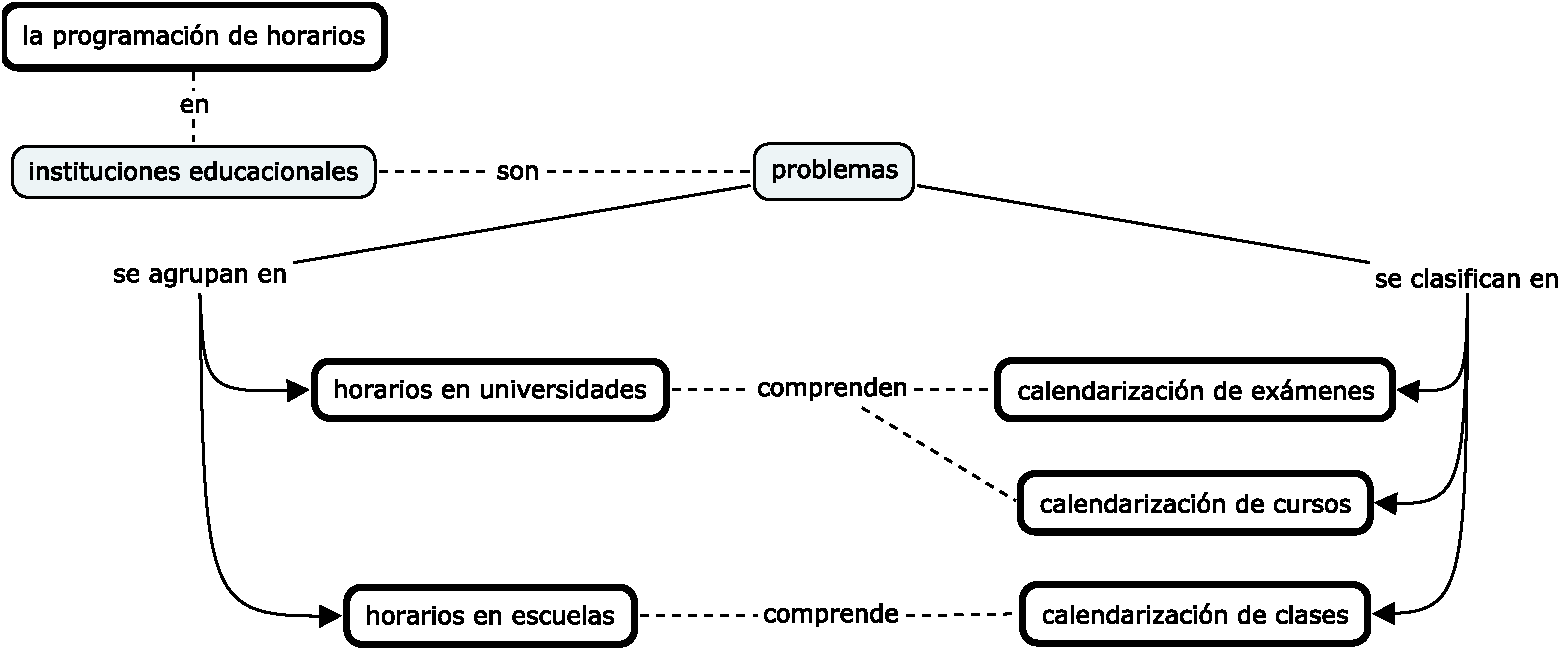
\includegraphics[width=.8\textwidth, trim=0 140 0 140]{timetabling_classification.pdf}
\caption[Clasificación del problema]{Clasificación de los problemas en la elaboración de horarios educacionales}
\label{fig:timetabling_classification}
\end{figure}

\iffalse
Classification of Educational Timetabling Problems
Schaerf (1999a) classified educational timetabling into three main classes i.e. school timetabling, course timetabling and examination timetabling. They share the same basic characteristics of the general timetabling problem but can still have significant differences between them. Each one of them has its own constraints, requirements and rules. More details on educational timetabling can be found in Burke et al. (2004e). In this section, a classification of educational timetabling and its properties are discussed. We divided educational timetabling into two categories i.e. school timetabling and university timetabling (which consists of examination timetabling and course timetabling).
\fi

\subsection{Horarios en escuelas}

\index{horarios!en escuelas}

\subsubsection{Horarios de clases}

\index{horarios!de clases}
De acuerdo a \citet[p.~88]{schaerf99a-survey-of-automated} el problema de horarios de clases consiste en calendarizar en un periodo semanal todas las clases de una escuela, evitando que los profesores se encuentren con dos clases al mismo tiempo, y viceversa. \citet[p.~10,11]{abdullah06heuristic-approaches} elabora explicando que el problema consiste de un conjunto de profesores, clases, lecciones y periodos semanales. En donde tales periodos semanales son predefinidos.

El problema intenta asignar lecciones a periodos y, un profesor a una clase en particular en un momento dado mientras se satisface un conjunto de limitaciones con el fin producir un horario factible. Algunos ejemplos de limitaciones en este tipo de problemas son las capacidades de alojamiento, ubicaciones, cargas de trabajo de los profesores, tiempo de descanso entre lecciones.

\iffalse
School timetabling: The weekly scheduling for all the classes of a school, avoiding teachers meeting two classes at the same time, and vice versa;

2.3.1 SchoolTimetabling
The school timetabling problem is concerned with the weekly scheduling for all the lessons of a school. The problem consists of a set of teachers, classes, subject/lessons and weekly periods. These weekly periods are predefined. This problem tries to assign lessons to periods and, a teacher to a particular class at a given time while satisfying a set of constraints in order to produce a feasible timetable.

Some examples of constraints in the school timetabling problem are capacities, locations, teacher loads, rest time between two lessons and other personal preferences. Examples of research on school timetabling can be found in Abramson (1991) who employed simulated annealing, Carrasco and Pato (2001) who employed a multi- objective genetic algorithm and Legierski (2003) who applied a constraint-based approach.
\fi

\subsection{Horarios en universidades}

\index{horarios!en universidades}\index{calendarización!de cursos}\index{calendarización!de exámenes}
El problema de la planificación de horarios en universidades puede ser agrupado en dos categorías: (i) calendarización de cursos y (ii) calendarización exámenes.
El problema de la calendarización de cursos es el proceso de la asignación de periodos y aulas de manera tal que las reuniones entre conferenciantes y estudiantes pueda ocurrir.
El problema de la calendarización de exámenes se refiere a la asignación de periodos y aulas de manera tal que los estudiantes puedan presentar sus exámenes.
Ambos problemas son similares de manera superficial, pero existen diferencias importantes que los distinguen.
En la calendarización de exámenes, múltiples exámenes pueden ser presentados en una misma aula (ej. auditorio) al mismo tiempo.
Sin embargo, esto no es posible para la calendarización de cursos en donde únicamente un curso puede ser asignado a un aula \citep[p.~11]{abdullah06heuristic-approaches}.

\iffalse
The university timetabling problem can be grouped into two categories: (i) course (or lecture) timetabling and (ii) examination timetabling. The course timetabling problem is the process of assigning timeslots and rooms so that meetings between lecturers and students can take place. The examination timetabling problem refers to the assignment of timeslots and rooms so that students can take examinations. These two (examination and course) timetabling problems are fairly similar in some superficial ways, but there are some distinct underlying differences between them. In examination timetabling, several examinations can be assigned to one (large) room at the same time. However, this is not possible for course timetabling where only one course can be assigned to one room.
\fi

\subsubsection{Calendarización de exámenes}

\index{calendarización!de exámenes}\index{calendarización!de cursos}
\citet[p.~4]{carter95recent-developments} definió el problema como la asignación de exámenes a un número limitado de periodos de manera tal que no existan conflictos o coincidencias. Los problemas de calendarización de cursos y exámenes son similares pero algunas diferencias relevantes según \citet[p.~159]{werra85an-introduction-to-timetabling} son:
\begin{enumerate}[a]
\item Existe generalmente un solo exámen por cada tema (mientras que hay varias exposiciones en un curso)
\item En la calendarización semanal de cursos, el objetivo principal es evitar conflictos (ej. la ocurrencia de que dos cursos elegidos por un mismo estudiante sean programados en el mismo periodo). Para los exámenes, generalmente se pide un máximo de un examen por día para cada estudiante o de ser posible, evitar la calendarización de exámenes en días consecutivos si el periodo de evaluación de exámenes lo permite.
\end{enumerate}
El problema de la calendarización de exámenes es muy común tanto en escuelas como en universidades. La asignación de los exámenes a los periodos está sujeta a un conjunto de limitaciones \citep[p.~12]{abdullah06heuristic-approaches}.

\iffalse
course sched- uling problems and exam scheduling problems were quite similar; bo:2 types could be formulated in terms of node coloring in a graph. There are in fact a few differences which should be underlined.
a) There is usually only one exam in each subject (while we had several lectures in a course). Exam graphs will so be generally smaller in size than course scheduling graphs.
b) In a weekly course schedvle, the only objec- tive is to avoid conflicts (i.e. the sJtuation where 2 courses chosen by a student are scheduled m ~he same period). For the exams, it is usua]iy required to have at most one exam per day for each student or even to avoid having exams on consecutive days if the time interval for exams atlows it.

Examination timetabling: The scheduling for the exams of a set of univer- sity courses, avoiding overlap of exams of courses having common students, and spreading the exams for the students as much as possible.

11Chapter 2. A Review of University Timetabling Problems and Approaches
Carter and Laporte (1996) defined the examination timetabling problem as:
“The assigning of examinations to a limited number of available time periods in such a way that there are no conflicts or clashes”
The examination timetabling problem is very common in both schools and universities. It is concerned with allocating a set of examinations, into a limited number of timeslots (periods), subject to a set of constraints. Carter et al. (1994) quoted that the basic challenge of examination timetabling is to schedule examinations over a limited number of timeslots so as to avoid conflicts and to satisfy a number of side constraints. In this case, the conflict is referred to as a hard constraint and side constraints are referred to as soft constraints.
\fi

\subsubsection{Calendarización de cursos}

\index{calendarización!de cursos}
El problema de la calendarización de cursos surge cuando una universidad (o incluso una escuela) ofrece una colección de cursos (cada uno consistiendo de un número dado de conferencias) sin existir un currículo fijo y en donde cada estudiante puede elegir cierto número de cursos. El problema consiste en la asignación de cada lectura a algún periodo en la semana de manera tal que ningún estudiante requiera asistir a más de una conferencia a la vez \citep[p.~157]{werra85an-introduction-to-timetabling}.
\citet[p.~88]{schaerf99a-survey-of-automated} define el problema como la calendarización semanal de todas las lecciones de un conjunto de cursos universitarios, minimizando los empalmes de las lecciones de cursos teniendo estudiantes en común.

\iffalse
The course scheduling problem arises when a university (or even a school) offers a collection of courses (each one consisting of a given number of lectures) and there is no fixed curriculum: Each student may choose a certain number of courses. The problem consists in assigning each lecture to some period of the week in such a way that no student is required to take more than one lecture at a time. {werra85an-introduction-to-timetabling}

Course timetabling: The weekly scheduling for all the lectures of a set of university courses, minimizing the overlaps of lectures of courses having common students;{schaerf99a-survey-of-automated}
\fi

\section{Horarios de clases}

\section{Calendarización de cursos}

\section{Calendarización de exámenes}

\chapter{Preliminares}

\section{Introducción}

\section{Historia de la calendarización}

\section{Terminología y definiciones}

\section{Complejidad computacional}

\subsection{Clases P y NP}

\chapter{Modelos matemáticos}

\section{Introducción}

\section{planificación de horarios en escuelas}

\section{Calendarización de cursos}

\section{Calendarización de exámenes}

\section{Un lenguaje en común}

\section{Algoritmos de solución}

\chapter{restricciones y funciones objetivo}

\section{Introducción}

\section{restricciones}

\section{Funciones objetivo}

\chapter{El gestor escolar}

\section{Aplicaciones}

\subsection{Métricas de desempeño}

\subsection{Multidisciplinario}

\section{Factores de interés}

\subsection{Laborales}

\subsubsection{Regulatorios}

\subsection{Diagnóstico}

\subsubsection{Interinstitucional}

\subsection{Inversión}

\subsubsection{Downsizing}

\subsection{Económicos}

\subsubsection{Utilidades}

\subsubsection{Fiscales}

\subsubsection{Aprovechamiento de recursos}

\subsection{Sociales}

\subsubsection{Involucramiento de paterfamilias}

\subsection{Institucionales}

\subsubsection{Profesorado}

\subsection{Flexibilidad}

\chapter{Herramientas de solución}

\section{Tipo de herramientas}

\subsection{Automatizadas}

\subsection{Interactivas}

\section{Listado de software}

\subsection{KHE}

\subsubsection{Formato de datos}

\chapter{Trabajo en el futuro y conclusiones}

\section{Resumen del trabajo de investigación}

\section{Contribuciones}

\section{Trabajo futuro}

\section{Diseminación}

\index{timetabling!university|see{programación de horarios en universidades}}
\index{timetabling!school|see{calendarización de clases y programación de horarios en escuelas}}
\index{timetabling!course|see{calendarización de cursos}}
\index{timetabling!examination|see{calendarización de exámenes}}

\index{scheduling|see{programación}}
\index{timetabling|see{programación de horarios}}

% Bibliography
\bibliographystyle{apalike}
\bibliography{/Users/harciga/Dropbox/bibliographies/reviewed,/Users/harciga/Dropbox/bibliographies/Dissertation_books}
{
\RaggedRight
\printindex
}
\end{document}
